\section{Auswertung}
\label{sec:Auswertung}

\subsection{Messung ohne Rauschen}
\label{sec:ohne rauschen}

\begin{figure}
  \begin{subfigure}{0.48\textwidth}
    \centering
    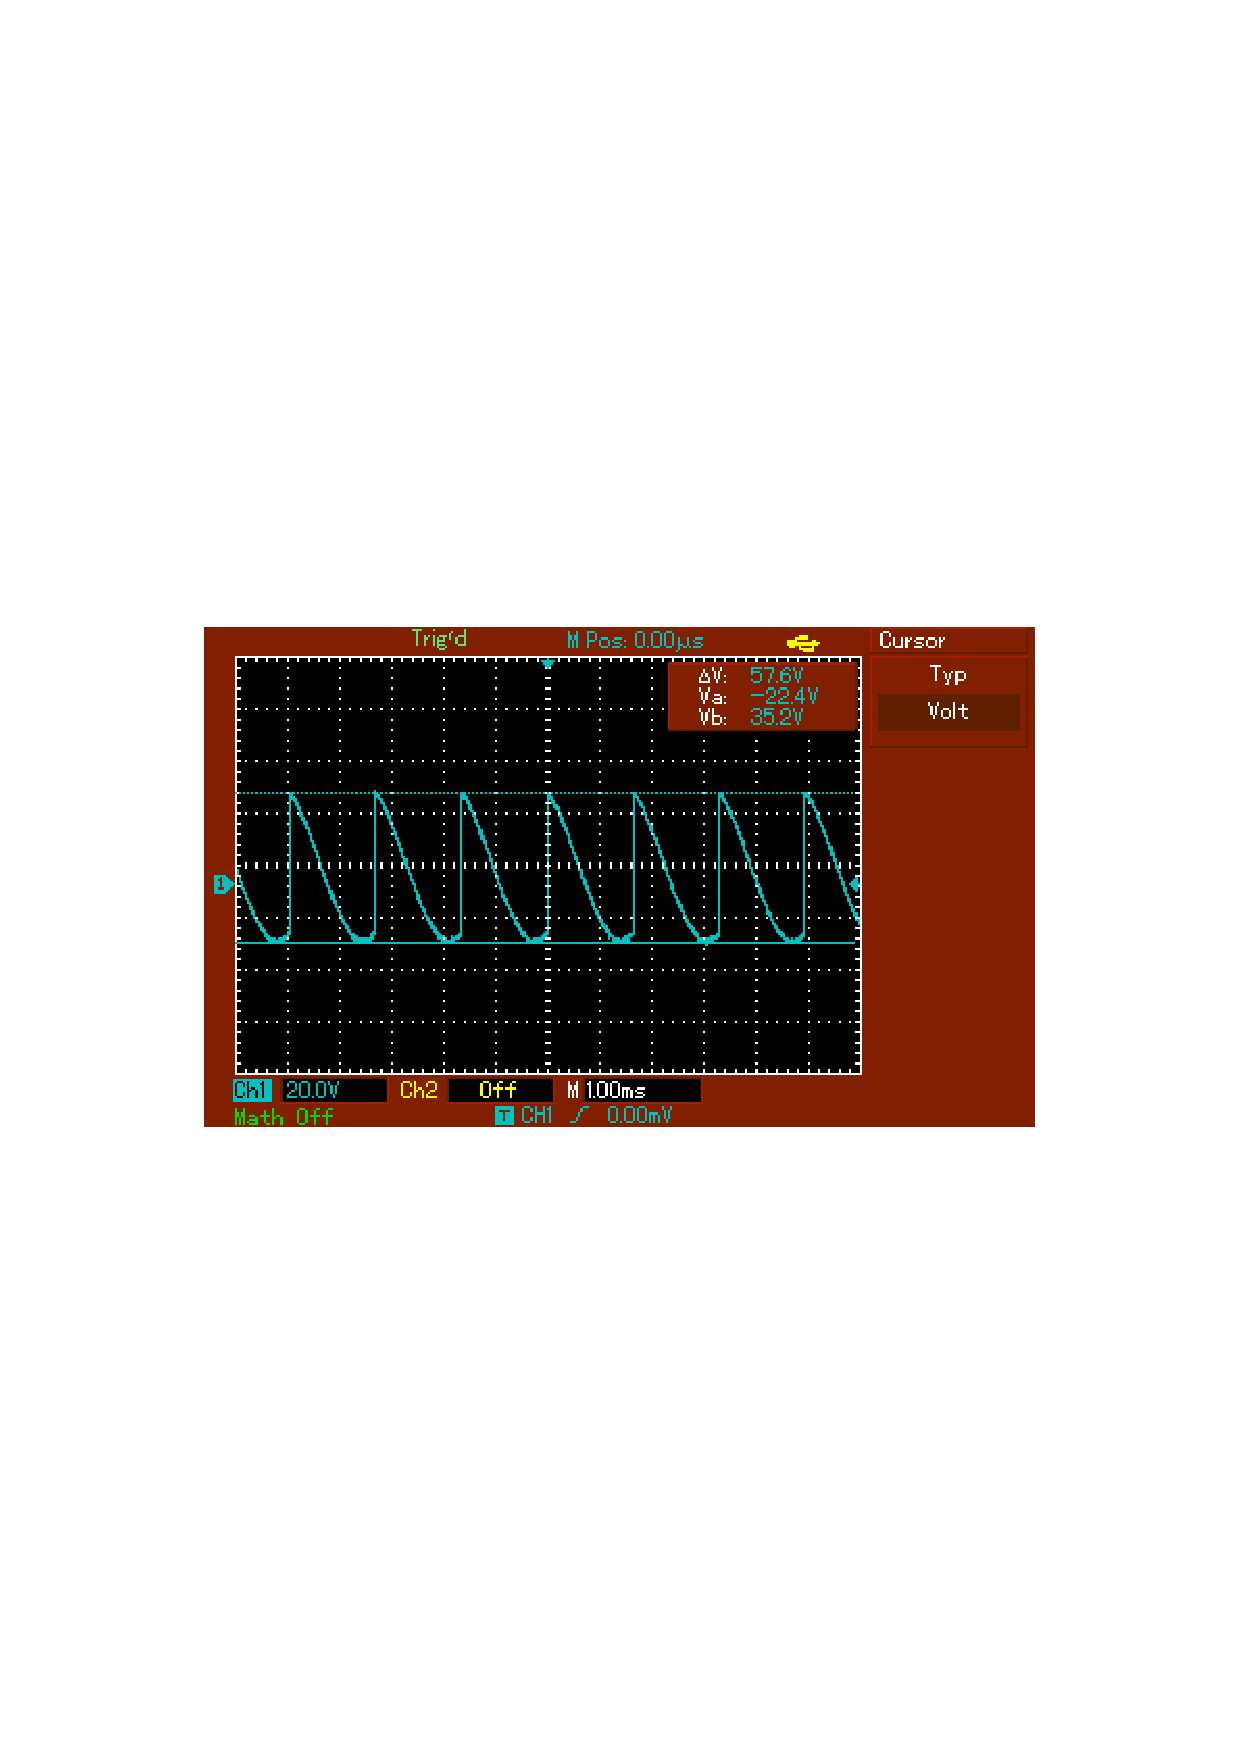
\includegraphics[height=4cm]{content/Bilder/unverrauscht/0.pdf}
    \caption{$\symup{\Delta}\varphi = \qty{0}{\degree}$}
  \end{subfigure}
  \begin{subfigure}{0.48\textwidth}
    \centering
    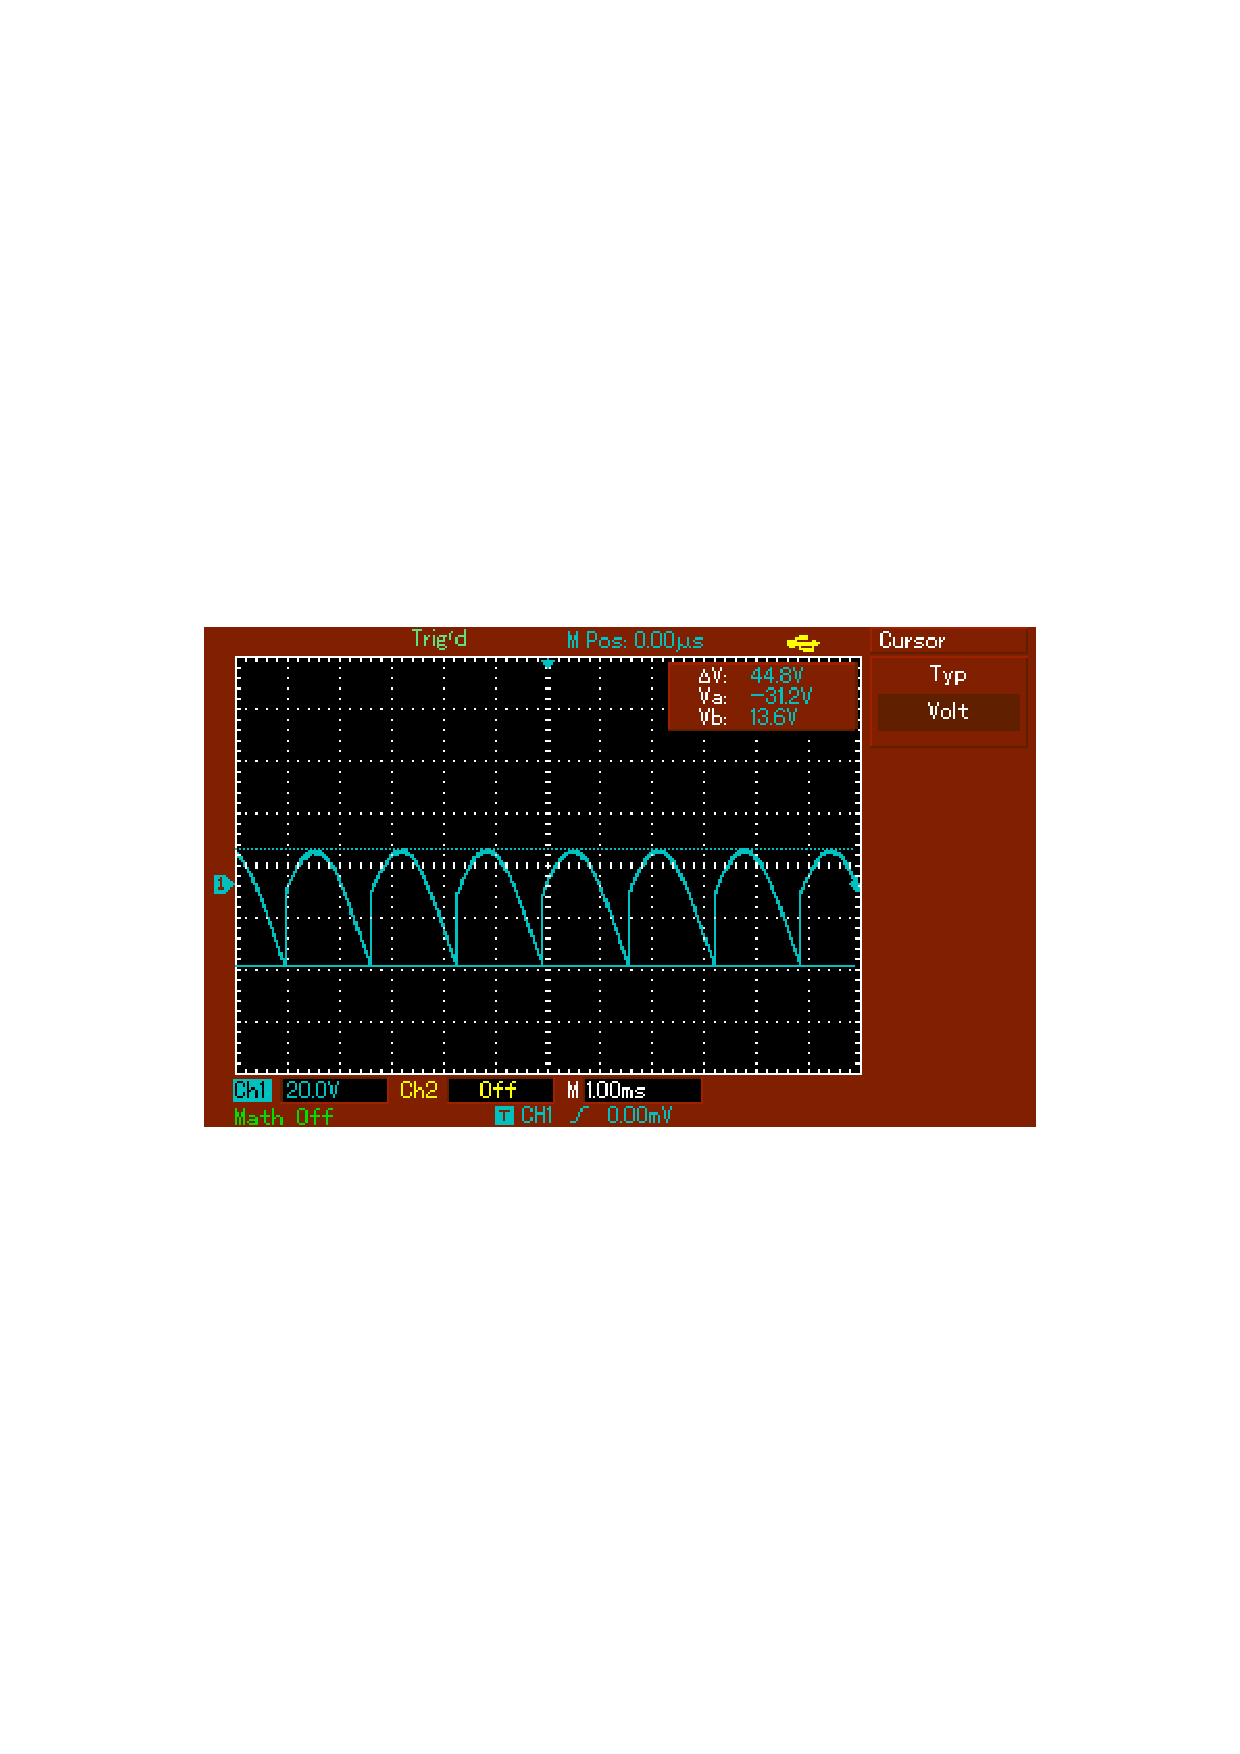
\includegraphics[height=4cm]{content/Bilder/unverrauscht/90.pdf}
    \caption{$\symup{\Delta}\varphi = \qty{90}{\degree}$}
  \end{subfigure}
  \begin{subfigure}{0.48\textwidth}
    \centering
    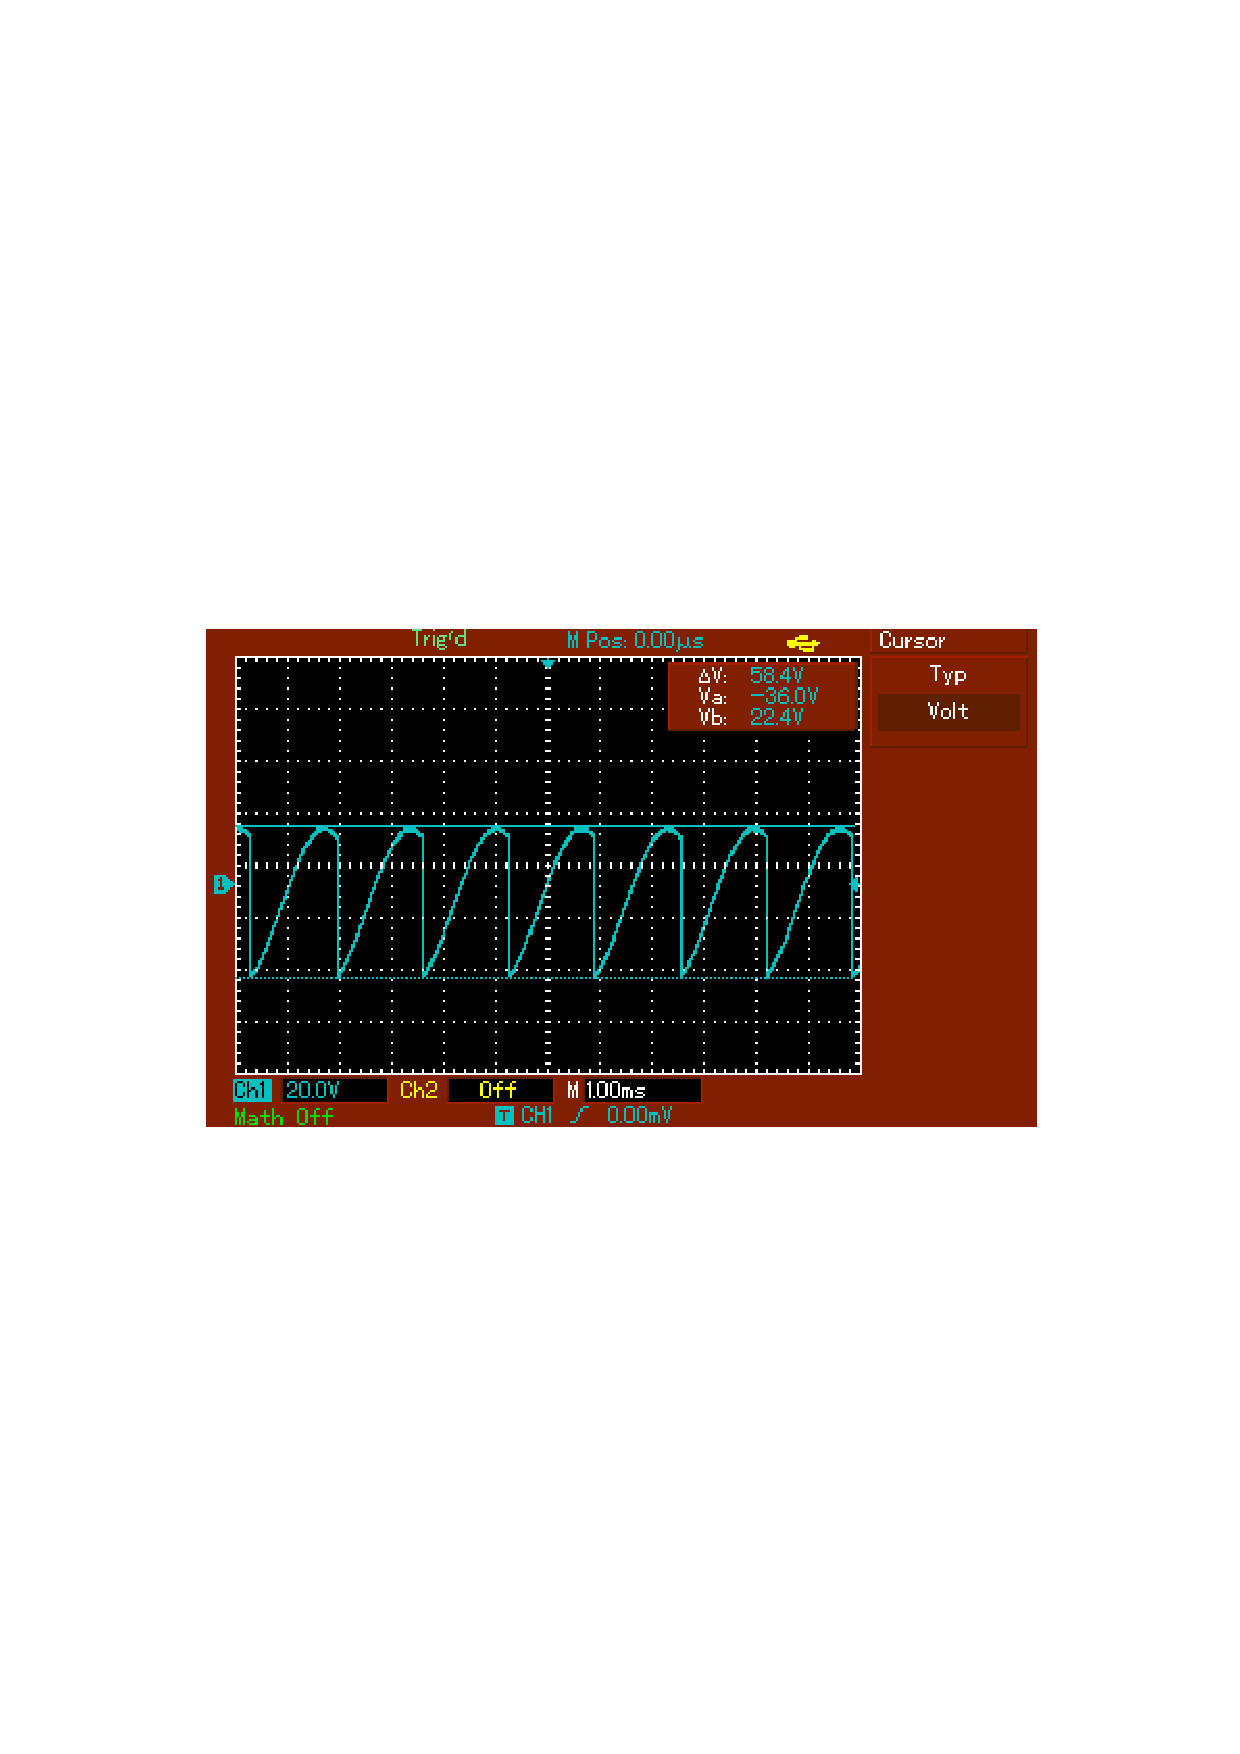
\includegraphics[height=4cm]{content/Bilder/unverrauscht/180.pdf}
    \caption{$\symup{\Delta}\varphi = \qty{180}{\degree}$}
  \end{subfigure}
  \begin{subfigure}{0.48\textwidth}
    \centering
    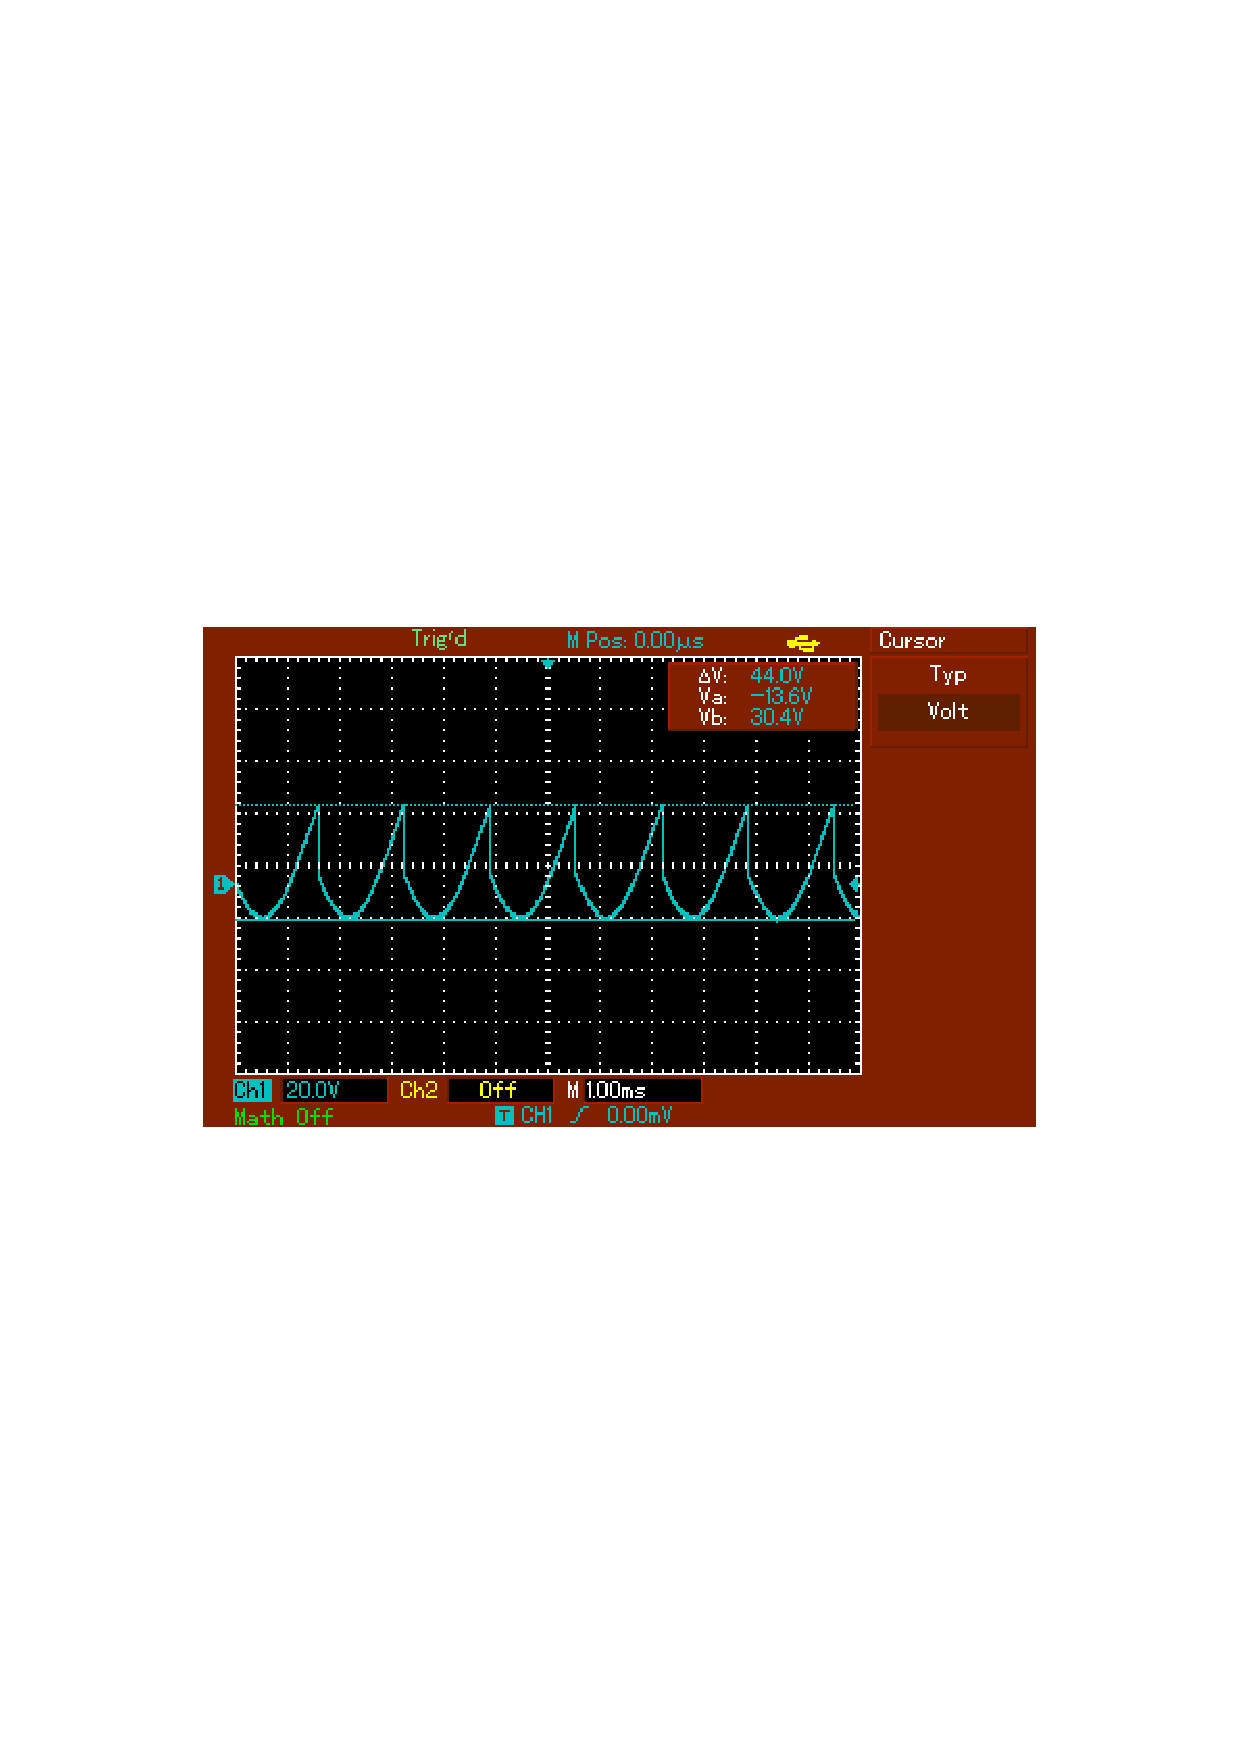
\includegraphics[height=4cm]{content/Bilder/unverrauscht/270.pdf}
    \caption{$\symup{\Delta}\varphi = \qty{270}{\degree}$}
  \end{subfigure}
  \begin{subfigure}{0.48\textwidth}
    \centering
    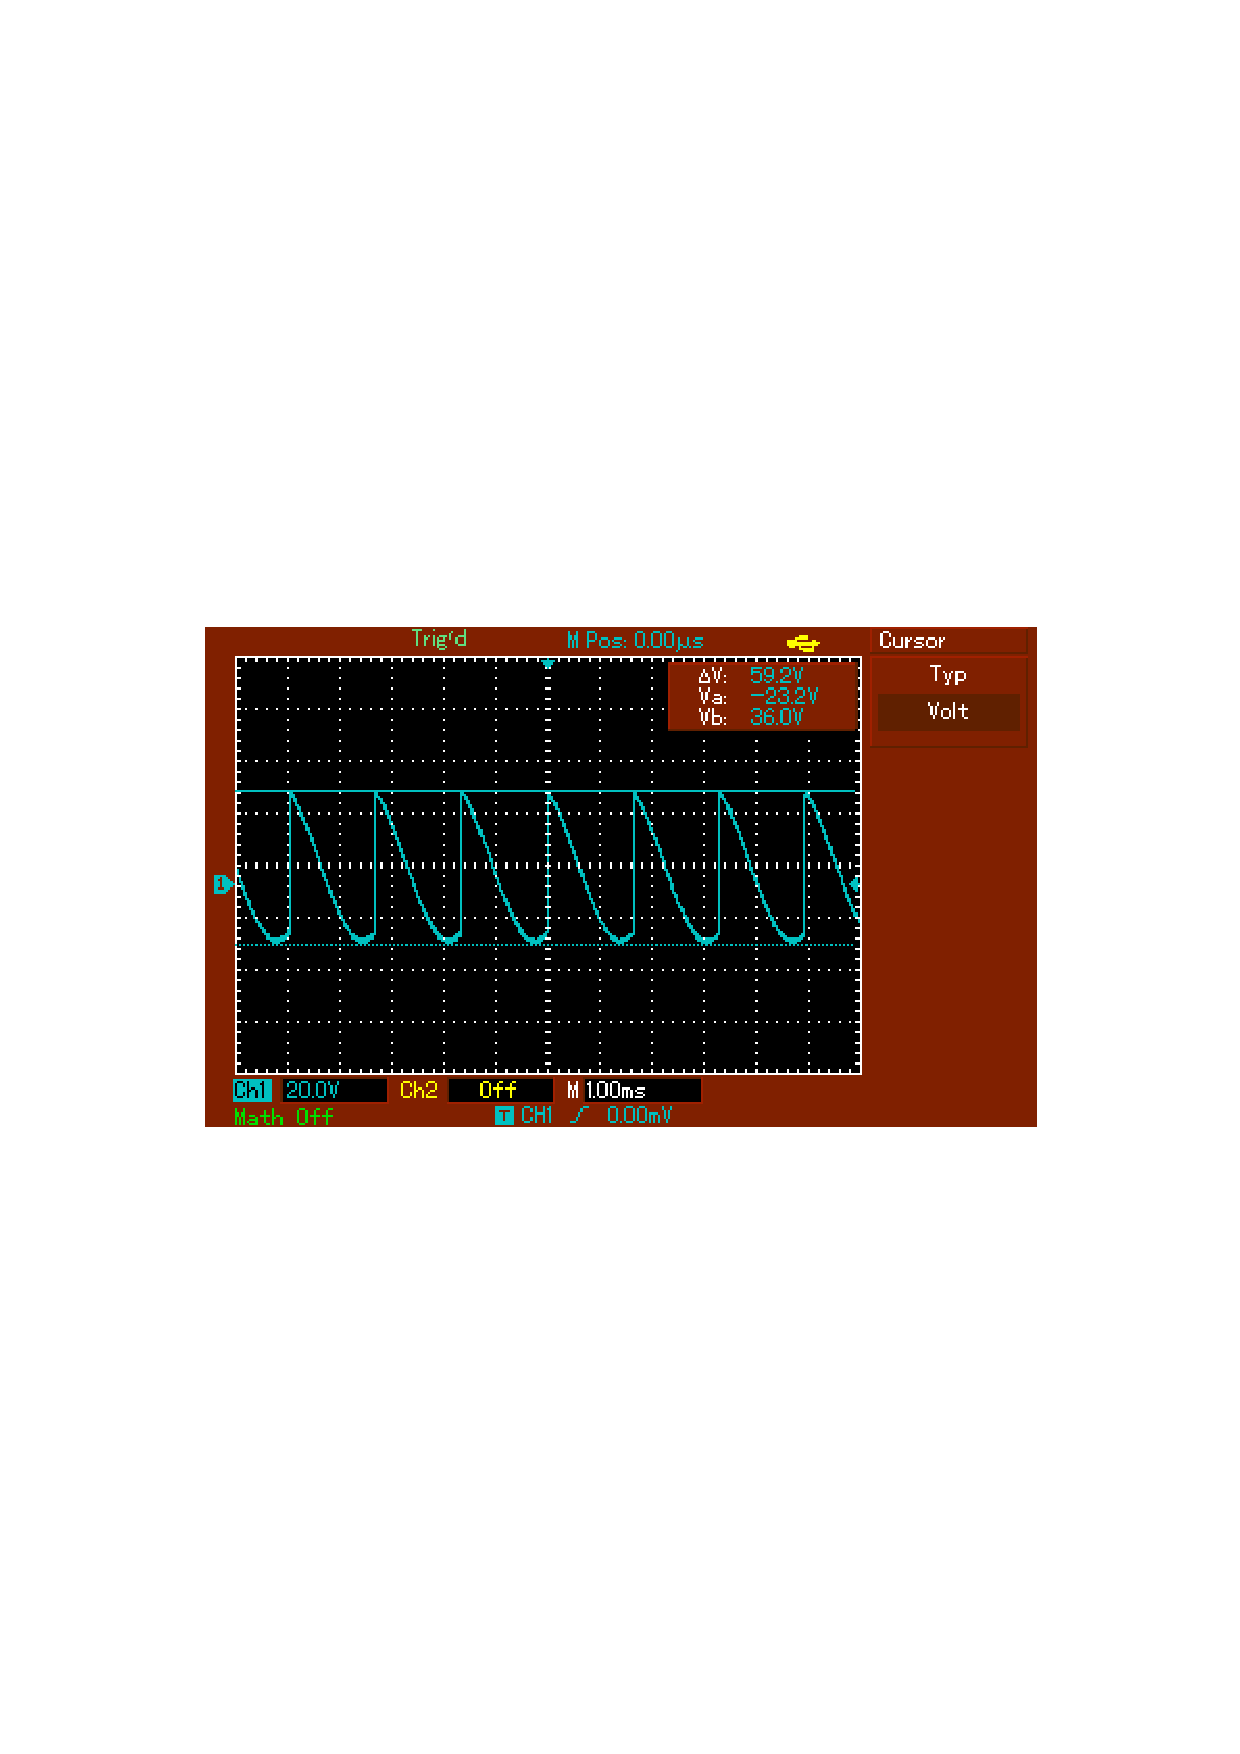
\includegraphics[height=4cm]{content/Bilder/unverrauscht/360.pdf}
    \caption{$\symup{\Delta}\varphi = \qty{360}{\degree}$}
  \end{subfigure}
  \caption{Oszilloskopbilder des Ausgabesignals $U_{\symup{sig}}$ für verschiedene Phasenverschiebungen $\symup{\Delta}\varphi$.}
  \label{fig:test}
\end{figure}

\begin{table} [H]
  \centering
  \caption{Amplitude des unverrauschten Signals in Abhängigkeit der Phasenverschiebung $\symup{\Delta}\varphi$}
  \label{tab:unverrauscht}
  \begin{tabular}{S[table-format=3.0] S[table-format=2.1]}
    \toprule
    {$\symup{\Delta}\varphi$} & {$U_{\symup{sig}}\,/\,\unit{\volt}$} \\
    \midrule
    0	  & 57.6 \\
    30	& 60.6 \\
    60	& 53.6 \\
    90	& 44.8 \\
    120	& 32.0 \\
    150	& 50.4 \\
    180	& 58.4 \\
    210	& 61.6 \\
    240	& 53.6 \\
    270	& 44.0 \\
    300	& 32.0 \\
    330	& 50.4 \\
    360	& 59.2 \\
    \bottomrule
  \end{tabular}
\end{table}

\begin{figure}
  \centering
  \includegraphics{build/plot_normal.pdf}
  \caption{Amplitude des Ausgangssignal $U_{\symup{sig}}$ vor dem Tiefpass in Abhängigkeit der Phasenverschiebung~$\varphi$.}
  \label{fig:plot normal}
\end{figure}

% Subsection mit Rauschen
\subsection{Messung mit Rauschen}
\label{sec:mit rauschen}

\begin{table} [H]
  \centering
  \caption{Amplitude des verrauschten Signals in Abhängigkeit der Phasenverschiebung~$\symup{\Delta}\varphi$}
  \label{tab:verrauscht}
  \begin{tabular}{S[table-format=3.0] S[table-format=1.2]}
    \toprule
    {$\symup{\Delta}\varphi$} & {$U_{\symup{sig}}\,/\,\unit{\volt}$} \\
    \midrule
    0	  & 1.52 \\
    30	& 1.28 \\
    60	& 1.14 \\
    90	& 0.92 \\
    120	& 1.02 \\
    150	& 1.26 \\
    180	& 1.80 \\
    210	& 1.42 \\
    240	& 1.16 \\
    270	& 1.00 \\
    300	& 1.58 \\
    330	& 1.62 \\
    360	& 1.88 \\
    \bottomrule
  \end{tabular}
\end{table}

% Subsection LED
\subsection{Messung mit einer LED}
\label{sec:LED}

\begin{table} [H]
  \centering
  \caption{Signalstärke des Ausgabesignals des Photodetektors abhängig von dem Abstand $r$ zwischen LED und Photdetektor.}
  \label{tab:led}
  \begin{tabular}{S[table-format=2.1] S[table-format=3.1]}
    \toprule
    {$r\,/\,\unit{\centi\metre}$} & {$U_{\symup{sig}}\,/\,\unit{\volt}$} \\
    \midrule
    6.6	  & 210.0\\
    7.0	  & 194.0\\
    7.5	  & 170.0\\
    8.0	  & 138.0\\
    8.5	  & 110.0\\
    9.0	  & 93.6 \\
    9.5	  & 83.2 \\
    10.0	& 74.4 \\
    11.0	& 60.0 \\
    12.0	& 48.0 \\
    13.0	& 40.0 \\
    14.0	& 32.4 \\
    15.0	& 28.0 \\ 
    17.0	& 20.4 \\ 
    19.0	& 16.2 \\ 
    21.0	& 12.8 \\
    23.0	& 11.4 \\
    25.0	& 9.0  \\
    30.0	& 6.9  \\
    40.0	& 5.5  \\
    50.0	& 4.5  \\
    60.0	& 3.9  \\
    \bottomrule
  \end{tabular}
\end{table}


\begin{figure}
  \centering
  \includegraphics{build/plot_led.pdf}
  \caption{Amplitude der Signalstärke $U_{\symup{sig}}$ des Photodetektors abhängig von dem Abstand $r$ zwischen der LED und des Photodetektors.}
  \label{fig:plot led}
\end{figure}
